
\section{Transcritical flow without a shock over a bump}

This scenario exhibits transcritical flow without a shock over a bump.
This test is adapted from Goutal and Maurel~\cite{GM1997}.
The topography and the initial conditions are the same as those used in the subcritical flow as well as the transcritical flow with a shock (See the description given in the report on the subcritical flow and transcritical flow with a shock). The boundary conditions are different from those used in the subcritical flow test. Here we refer to the parameters used by Goutal and Maurel~\cite{GM1997}. The analytical height or depth $h$ of the transcritical flow is calculated the Bernoulli equation. The velocity is computed as $u=q/h$\,.

\subsection{Results}
Referring to Goutal and Maurel~\cite{GM1997}, we consider the initial condition
\begin{equation}
u(x,y,0)=v(x,y,0)=0\,, \quad
w(x,y,0)= 0.66\,,
\end{equation}
We enforce Dirichlet boundary conditions
at $x=0^{-}$ given by
\begin{equation}
[w,hu,hv]=[1.0144468506259066,~~~1.53,~~~0]\,,
\end{equation}
and at $25^{+}$ given by
\begin{equation}
[w,hu,hv]=[0.4057809296474606,~~~1.53,~~~0]\,.
\end{equation}




Representatives of the simulation results are given in the following three figures. We should see excellent agreement between the analytical and numerical solutions. Small discrepancy may occurs for the $x$-momentum. It is not clear what makes this discrepancy. Numerical analysis may be conducted further to investigate why this discrepancy occurs.

\begin{figure}
\begin{center}
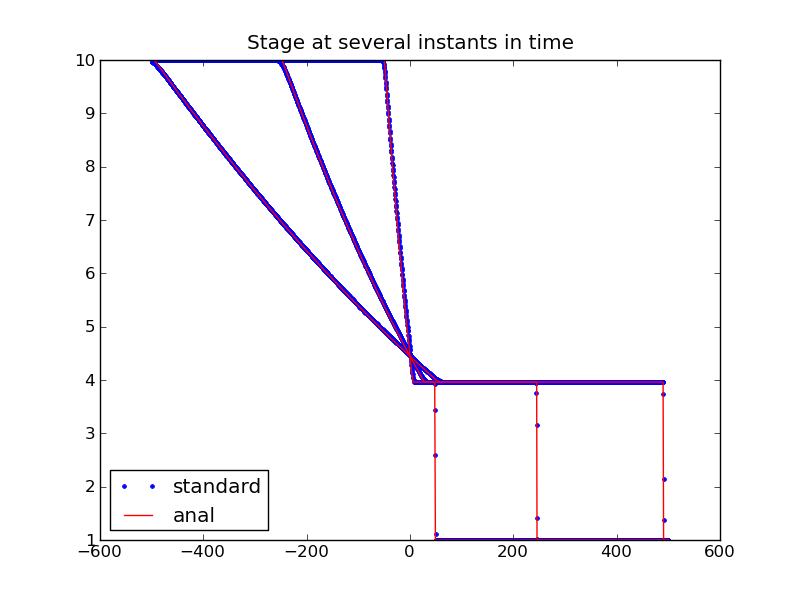
\includegraphics[width=0.9\textwidth]{stage_plot.png}
\end{center}
\caption{Stage results}
\end{figure}


\begin{figure}
\begin{center}
\includegraphics[width=0.9\textwidth]{xmom_plot.png}
\end{center}
\caption{Xmomentum results}
\end{figure}


\begin{figure}
\begin{center}
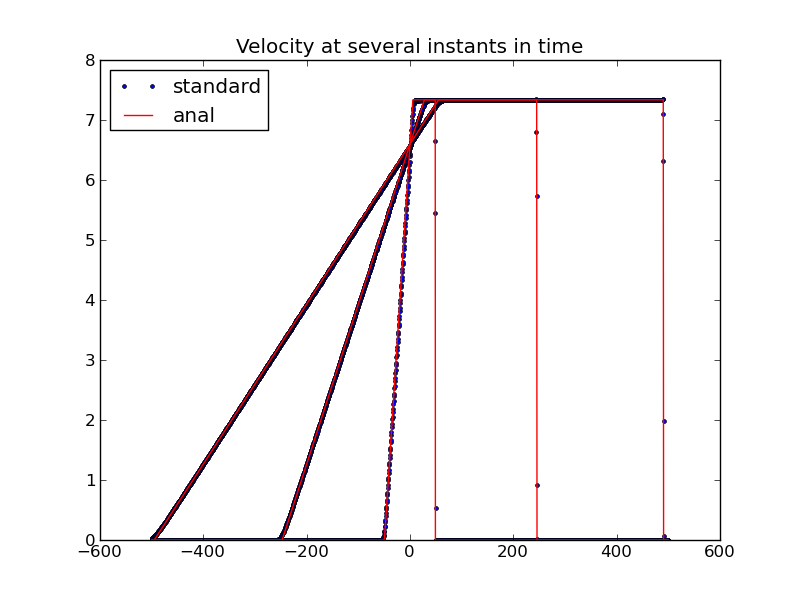
\includegraphics[width=0.9\textwidth]{xvel_plot.png}
\end{center}
\caption{Xvelocity results}
\end{figure}


\endinput
